\chapter{Frozen-controller acceleration and the combined cycle}
\label{ch:transfer}
These tests change the operating task after the earlier local controller development. The no-load ramp and common-sensor audit distinguish actual mechanical speed from the feedback measurement. The first combined cycle is a transfer test for the earlier frozen controllers; the same cycle later becomes a selection case for DOB98. Its evidential role therefore depends on the controller being discussed.

\section{Five-second no-load acceleration and the common-sensor audit}
\textit{Archived October study. All simulations, searches, and checks described below predate this report.}\par

\subsection*{Chapter overview}Four existing controllers are tested on the same nonlinear plant with zero external shaft extraction. The target rises from 9000 to 10000 rpm in five seconds. Base PI has the lowest ramp tracking error in this experiment. Ringing-aware PILCO improves ramp tracking relative to the previous PILCO, but does not outperform base PI. This is a transfer test of frozen policies, not a new training result.
\subsection{Identical-sensor audit and fresh rerun}
All four models explicitly use the same T-MATS first-order speed-sensor library block: time constant 0.05 s, unity gain, limits 0--20000 rpm, initial value from the same plant initial speed, noise disabled, unity fault gain and zero drift. The sensor sample-time setting is the same plant solve interval. Model wiring assertions verify that both the base PI and each active advanced controller receive this sensor output directly. The sensor input comes from the same plant-output block in every model.

The earlier models already had these settings. The new simulations explicitly enforce them in separate model copies and reproduce the earlier speed, sensed-speed and fuel traces. Thus the prior ranking was not caused by unequal sensor dynamics. Controllers respond differently to the same lag. During a ramp, actual-speed error and sensed-speed error differ; the primary tables continue to score actual shaft speed. Individual audit JSON files and a sensor-comparison CSV accompany the results.
\subsection{Reproducible test protocol}
Rated speed is defined as $N_{100}=10000$ rpm. With $\tau=t-60$ s, the reference is
\begin{equation}r(\tau)=9000+200\min\{5,\max\{0,\tau\}\}\quad\text{rpm}.\end{equation}
Thus the reference acceleration is $200$ rpm/s, or two percentage points of rated speed per second. External PTO load is identically zero. The compressor still consumes shaft power: no external load does not mean zero internal torque.

The plant starts at 10000 rpm, ramps down during absolute time 5--10 s, and settles at 9000 rpm before the evaluation begins at 60 s. Controller handover is at 45 s. All four traces are within 0.1 rpm of 9000 rpm throughout the final five seconds before the test. The requested acceleration occurs at absolute time 60--65 s; simulation continues to 80.01 s. Sea-level, ISA-zero, Mach-zero settings are shared. The reference governor permits 200 rpm/s.

Logged samples are spaced by 0.015 s. The continuous target ramp lasts exactly 5 s; its first post-end sample is at $\tau=5.01$ s. Maximum logged-reference discrepancy from the equation above is below $2\times10^{-12}$ rpm. Every saved sample passes the existing model-validity flag, and every external-load sample is zero.

\subsection{Controllers held fixed}
\begin{center}\small\begin{tabular}{lrrr}\toprule Controller & $K_p$ & $K_i$ & $K_d$\\\midrule
Base PI & .025 & .050 & 0\\
Retuned Poly2 + PID & .025 & .140 & .00125\\
Previous PILCO & .06460568 & .17102610 & 0\\
Smooth PILCO & .02479762 & .05385920 & 0\\\bottomrule\end{tabular}\end{center}
Both PILCO-style policies retain the prior quadratic feedforward, PI feedback, saturation and anti-windup implementation. Their nominal command structure is
\begin{align}u_k^*&=p_2(r_k,0,T_k,P_k)+K_p(r_k-N_{s,k})+I_k,\\
u_k&=\operatorname{clip}(u_k^*,0.2,4.0),\qquad
I_{k+1}=I_k+hK_i(r_k-N_{s,k}),\end{align}
with conditional integration at saturation. The zero second feedforward argument is retained from the prior controller, including during acceleration. No acceleration feedforward term is newly fitted for this test. The Poly2 PID comparator retains its previous inverse-model/derivative implementation; it is not replaced by the PILCO PI law.
\subsection{Measured response}
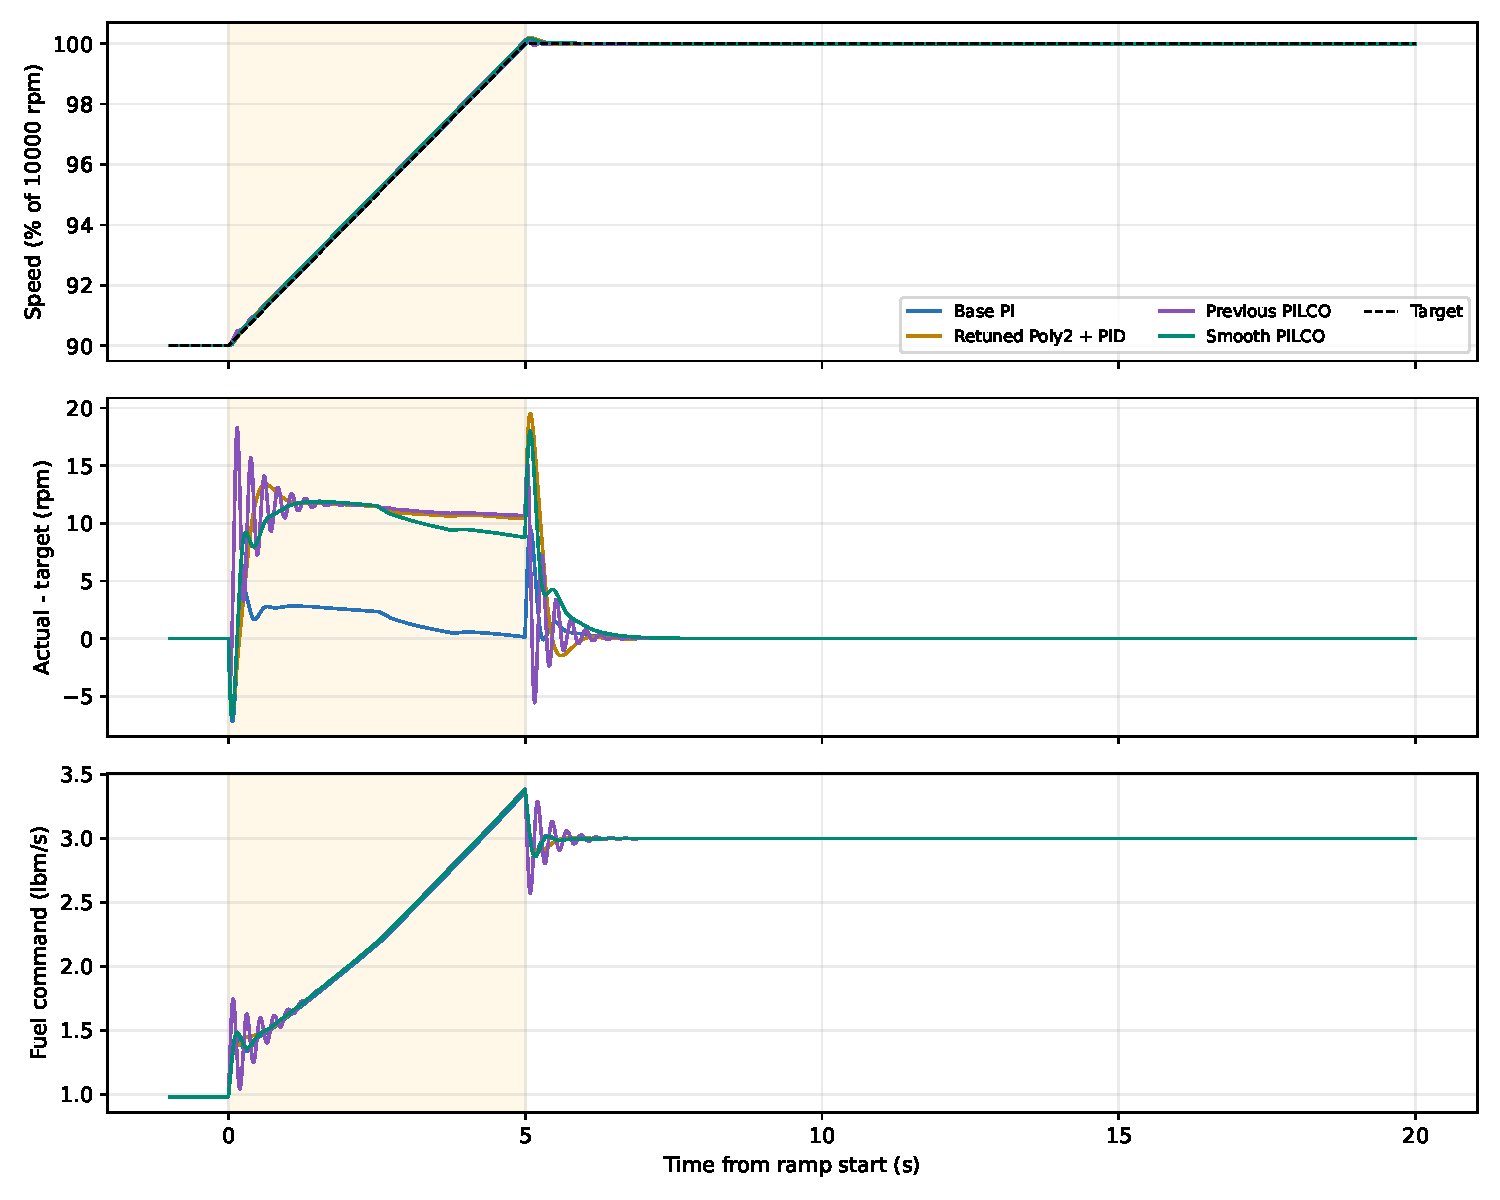
\includegraphics[width=\textwidth,height=.68\textheight,keepaspectratio]{late2_responses.pdf}
The pale band marks the five-second target ramp. Curves are raw recorded simulation traces; no display smoothing is used. Speed curves nearly overlap at the full-speed scale, so the signed error panel is needed to distinguish tracking performance.
\subsection{Quantitative comparison}
For each sample, $e_k=N_k-r_k$. Ramp RMSE uses $0\leq\tau<5$ s; full RMSE uses $0\leq\tau\leq20.01$ s. Settling is measured after ramp completion: the first recorded time after which every remaining sample stays within $\pm1$ rpm of 10000 rpm, minus 5 s. It is a finite-record measurement.
\begin{center}\small\begin{tabular}{lrrrr}\toprule
Controller & Ramp RMSE & Full RMSE & Peak $|e|$ & Settle\\
 & rpm & rpm & rpm & s after ramp\\\midrule
Base PI & 2.161 & 1.309 & 9.42 & 0.610 \\
Retuned Poly2 + PID & 10.949 & 5.799 & 19.54 & 0.760 \\
Previous PILCO & 11.224 & 5.710 & 18.31 & 0.820 \\
Smooth PILCO & 10.252 & 5.392 & 18.00 & 1.045 \\
\bottomrule\end{tabular}\end{center}
Fuel excess total variation is
\begin{equation}R_u=\sum_{k=a+1}^{b}|u_k-u_{k-1}|-|u_b-u_a|.\end{equation}
It measures movement beyond net endpoint change, in lbm/s, not fuel consumption. For acceleration, some excess variation is physically useful: fuel may rise to accelerate and then drop to its steady value. Therefore the whole-test measure is not a pure measure of unwanted oscillation. A separate post-ramp value is included. These intervals differ from the earlier load-pulse study; their totals must not be compared directly.
\begin{center}\small\begin{tabular}{lrrrr}\toprule
Controller & Whole $R_u$ & Post-ramp $R_u$ & Overshoot & Min. surge\\
 & lbm/s & lbm/s & rpm & \%\\\midrule
Base PI & 1.2188 & 0.2895 & 9.42 & 13.98 \\
Retuned Poly2 + PID & 1.0004 & 0.2189 & 19.54 & 13.74 \\
Previous PILCO & 6.2413 & 2.6423 & 15.23 & 13.74 \\
Smooth PILCO & 1.3489 & 0.3454 & 18.00 & 13.78 \\
\bottomrule\end{tabular}\end{center}
\subsection{Interpretation and limits}
Base PI gives the smallest ramp and full-evaluation RMSE. The smooth PILCO ramp RMSE is 10.252 rpm versus 11.224 rpm for the previous PILCO, an 8.7\% reduction. This does not establish a universal ranking: the earlier load-disturbance objective and the present acceleration objective are different.

PILCO gains were learned around 9250 rpm under load pulses. This ramp moves beyond that local operating condition; portions also lie beyond the approximately 9264--9750 rpm polynomial fitting range. The present result is evidence for this single deterministic nominal simulation, not a robustness guarantee. It does not validate the Gaussian-process model across the entire ramp or prove that a ringing penalty alone explains all differences between the gain sets.

The previous derivation remains applicable to how the gains were obtained: expected tracking and fuel-magnitude costs were augmented by expected excess fuel variation, using previous-command and segment-anchor memory. This run does not retrain that objective. A dedicated acceleration-training study would be needed to claim optimized ramp performance.
\subsection{Reproduction}
Run \path{ramp90_equal_sensor_batch.m} in MATLAB with the existing T-MATS dependencies. The four \path{GasTurbine_EqualSensor_*.mdl} copies preserve previous studies. Raw CSV/MAT traces and summary metrics are in \path{results/pilco_ramp90_equal_sensor_20261010}. Run \path{build_ramp90_equal_sensor.py} for this analysis and \path{build_ramp90_equal_sensor.py} for the synchronized video.


\section{Combined acceleration and a five-second load pulse}
\textit{Archived October study. All simulations, searches, and checks described below predate this report.}\par

\subsection{Requested cycle}
Define relative time $\tau=t-60$ s. The shaft-speed target and external load are
\begin{align}
r(\tau)&=9000+200\min(5,\max(0,\tau))\quad\mathrm{rpm},\\
P_L(\tau)&=\begin{cases}0.1P_{\rm ref},&10\le\tau<15,\\0,&\text{otherwise}.\end{cases}
\end{align}
The speed target ramps from 90\% to 100\% in five seconds, then remains at 10000 rpm. A common load is applied at second 10 and removed at second 15. Recovery is recorded through second 25.005. The five-second pulse is programmed as a zero-order-held workspace signal, with interpolation disabled.

The reference is the mean turbine shaft power at settled 10000 rpm from seconds 8--10 of the preceding no-load base-PI run: $P_{\rm ref}=27896.501$ hp. Therefore every controller receives exactly the same pulse amplitude, 2789.650 hp. This is 10\% of that common turbine-power reference, not 10\% of each controller's instantaneous power. Internal compressor power is still present.

The preparation stage begins at 10000 rpm, moves to 9000 rpm during absolute seconds 5--10, and settles before the cycle starts at absolute second 60. All cases use sea-level ISA-zero, Mach-zero conditions. Controller gains remain fixed. All four sensors have a 0.05 s time constant, unity gain, identical limits and initial conditions, and noise disabled. Wiring assertions confirm that each active controller receives the sensor output.

The model sample interval is 0.015 s. The first logged loaded sample is at relative 10.005 s, and the first unloaded sample is at 15.000 s. The programmed event interval is exactly 10--15 s; observed event timing is resolved on the sample grid. All simulations pass the existing model-validity checks.
\subsection{Comparison definitions}
Error means actual shaft speed minus target, $e_k=N_k-r_k$. Ramp RMSE uses $0\le\tau<5$ s; load/recovery RMSE uses $10\le\tau\le25.005$ s; full-cycle RMSE uses $0\le\tau\le25.005$ s. These are sample-weighted metrics. Scoring the two phases separately prevents the long recovery interval from concealing ramp differences.
\subsection{Recorded responses}
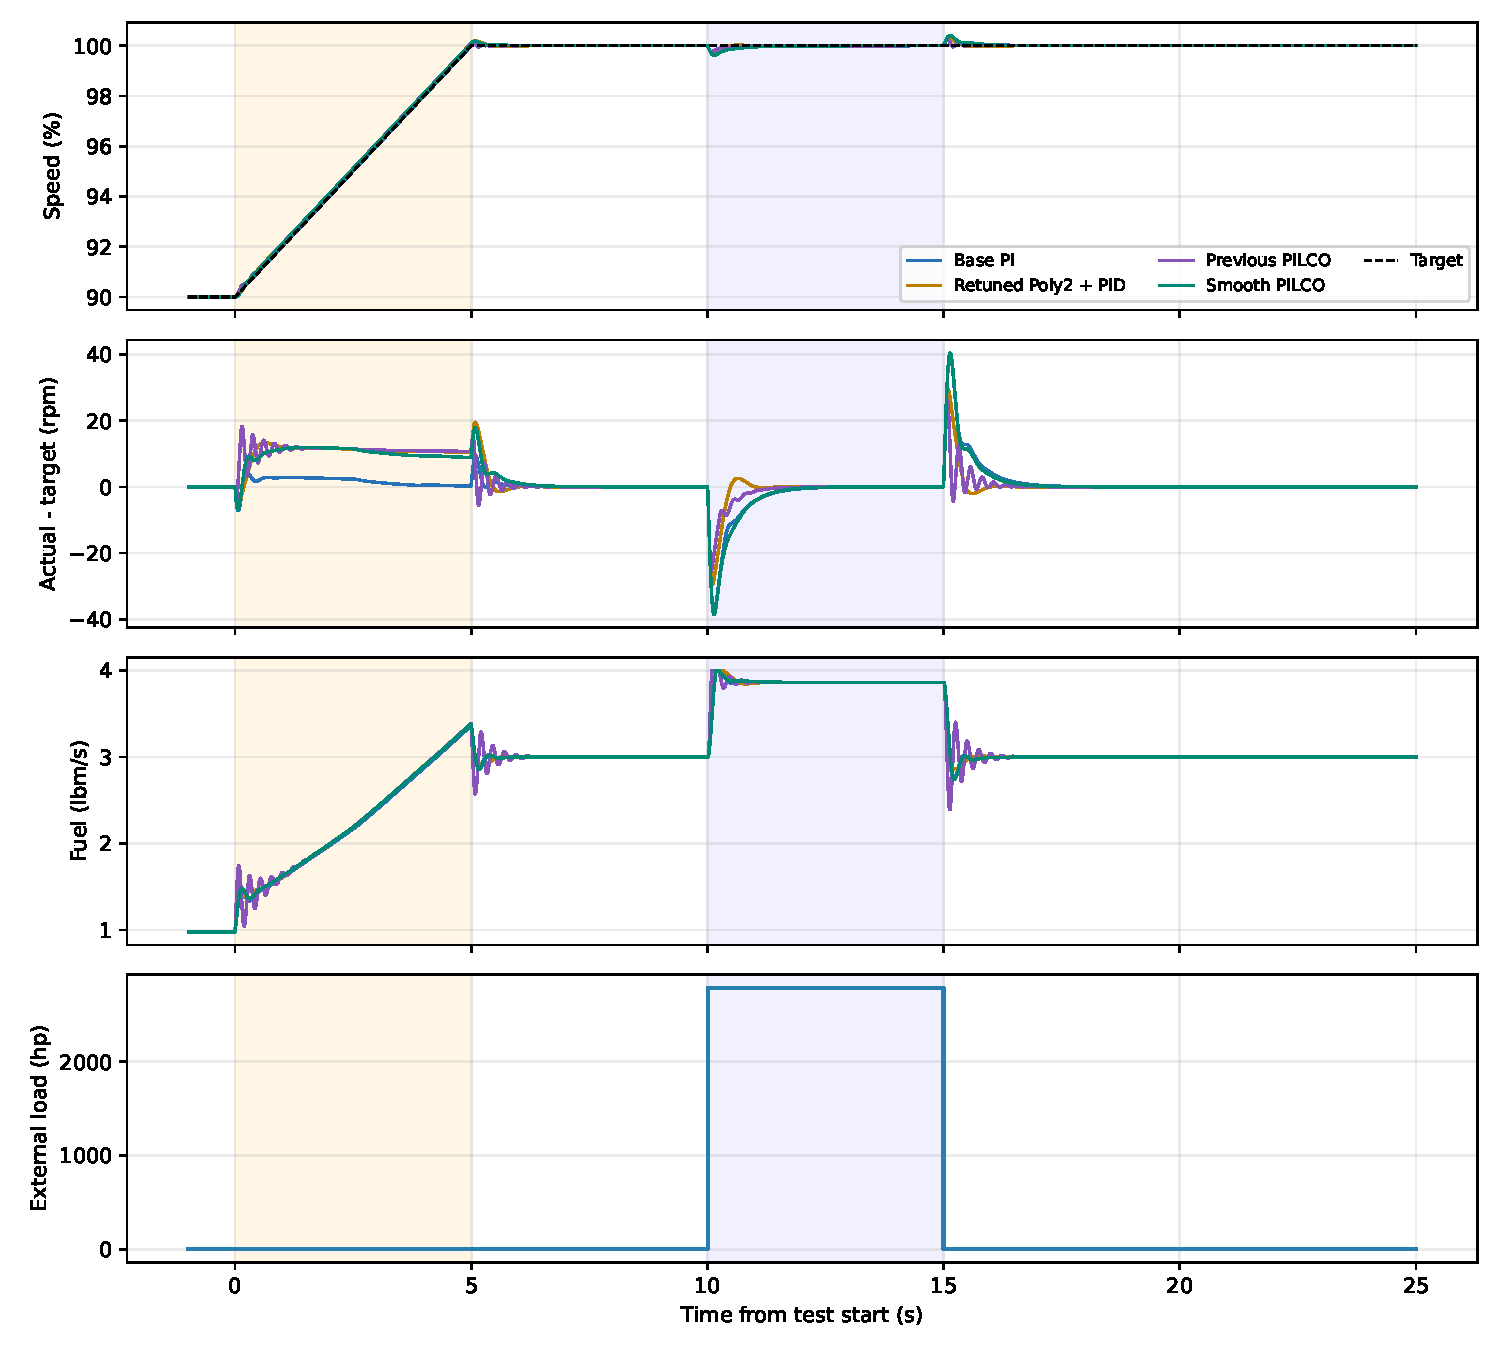
\includegraphics[width=\textwidth,height=.68\textheight,keepaspectratio]{late3_responses.pdf}
Orange shading marks the target ramp; blue shading marks the external-load pulse. These are raw nonlinear simulation traces, with no visual smoothing.
\subsection{Numerical results}
\begin{center}\small\begin{tabular}{lrrr}\toprule
Controller & Ramp RMSE & Load/recovery RMSE & Full RMSE\\ & rpm & rpm & rpm\\\midrule
Base PI & 2.161 & 6.815 & 5.408 \\
Retuned Poly2 + PID & 10.949 & 4.416 & 6.214 \\
Previous PILCO & 11.224 & 3.393 & 5.745 \\
Smooth PILCO & 10.252 & 6.913 & 7.207 \\
\bottomrule\end{tabular}\end{center}
\begin{center}\small\begin{tabular}{lrrrr}\toprule
Controller & Load peak $|e|$ & Fuel excess TV & Min. surge & Saturation\\
& rpm & lbm/s & \% & \% samples\\\midrule
Base PI & 40.13 & 0.945 & 7.64 & 0.7 \\
Retuned Poly2 + PID & 29.39 & 0.696 & 7.75 & 0.1 \\
Previous PILCO & 26.03 & 4.489 & 7.77 & 0.7 \\
Smooth PILCO & 40.47 & 0.919 & 7.63 & 0.2 \\
\bottomrule\end{tabular}\end{center}
Fuel excess total variation is $\sum|\Delta u|-|u_{\rm end}-u_{\rm start}|$, computed separately over 10--15 s and 15--25.005 s and then summed. It describes excess command movement, not fuel consumption. Minimum surge margin and fuel saturation are evaluated over the full cycle.

The previous and smooth PILCO policies use quadratic setpoint feedforward plus PI feedback. Retuned Poly2 retains its inverse-model/PID implementation; base PI remains the original baseline. No gains, feedforward coefficients or ringing weights were fitted to this combined cycle. These are nominal transfer-test results, not proof of robustness or global superiority. In particular, all controllers share the same sensor dynamics; differences in actual-speed tracking must not be attributed to unequal sensor time constants.
\subsection{Reproduction and saved outputs}
Run \path{combined_cycle_batch.m} in the existing MATLAB/T-MATS workspace. New models are named \path{GasTurbine_Combined_*.mdl}; earlier studies are preserved. Raw traces, model audit JSON, numerical metrics and the exact protocol are saved under \path{results/pilco_combined_cycle_20261010}. Analysis and video builders are \path{build_combined_cycle.py} and \path{build_combined_video.py}.


